\documentclass[12pt,a4paper]{scrartcl} 
\usepackage[utf8]{inputenc}
\usepackage[english,russian]{babel}
\usepackage{indentfirst}
\usepackage{misccorr}
\usepackage{graphicx}
\usepackage{indentfirst}
\usepackage{amsmath}
\usepackage{mathtools}
\usepackage{fancyhdr}
\usepackage{minted}
\setminted{
    style=emacs,
    breaklines=true,
    autogobble=true,
    linenos=true,
    frame=single,
    fontsize=\small
}

\begin{document}
 \begin{titlepage}
  \begin{center}
   \large
   МИНИСТЕРСТВО НАУКИ И ВЫСШЕГО ОБРАЗОВАНИЯ РОССИЙСКОЙ ФЕДЕРАЦИИ
   
   Федеральное государственное бюджетное образовательное учреждение высшего образования
   
   \textbf{АДЫГЕЙСКИЙ ГОСУДАРСТВЕННЫЙ УНИВЕРСИТЕТ}
   \vspace{0.25cm}
   
   Инженерно-физический факультет
   
   Кафедра автоматизированных систем обработки информации и управления
   \vfill

   \vfill
   
   \textsc{Отчет по практике}\\[2mm]
   
   {\LARGE Программная реализация вычисления матрицы обратную заданной
    \vspace{0.25cm}
   
   \textit{Вариант 5}}
   \bigskip
   
   1 курс, группа 1ИВТ1-1
  \end{center}
  \vfill
  
  \newlength{\ML}
  \settowidth{\ML}{«\underline{\hspace{0.7cm}}» \underline{\hspace{2cm}}}
  \hfill\begin{minipage}{0.5\textwidth}
   Выполнил:\\
   \underline{\hspace{\ML}} Д.\,А.~Лиев\\
   «\underline{\hspace{0.7cm}}» \underline{\hspace{2cm}} 2023 г.
  \end{minipage}%
  \bigskip
  
  \hfill\begin{minipage}{0.5\textwidth}
   Руководитель:\\
   \underline{\hspace{\ML}} С.\,В.~Теплоухов\\
   «\underline{\hspace{0.7cm}}» \underline{\hspace{2cm}} 2023 г.
  \end{minipage}%
  \vfill
  
  \begin{center}
   Майкоп, 2023 г.
  \end{center}
 \end{titlepage}
 
% Содержание
\section{Введение}
\label{sec:intro}


\subsection{Формулировка цели}
Целью данной работы является написание программы для нахождение обратной матрицы методом Гаусса.

\subsubsection{Теория}
В методе Гаусса (и его модификации, такой как метод Гаусса-Жордана), основной целью является приведение матрицы к улучшенному ступенчатому виду или диагональному виду. Это достигается путем применения элементарных преобразований строк матрицы.

Элементарные преобразования строк включают:
    \begin{enumerate}
        \item умножение на число, отличное от нуля;
        \item прибавление к элементам какой-либо строки или какого-либо столбца;
        \item перемена местами двух строк матрицы.
    \end{enumerate}
    \noindent 

Целью применения этих преобразований является создание нулевых элементов под главной диагональю или приведение матрицы к диагональному виду, что облегчает нахождение решений систем линейных уравнений или обратных матриц.

Использование метода Гаусса позволяет решать системы линейных уравнений и находить обратные матрицы путем последовательного применения элементарных преобразований строк матрицы до достижения требуемого вида.

\subsubsection{Практика}
Рассмотрим шаги по нахождению обратной матрицы методом Гаусса подробно:
\begin{enumerate}
        \item предположим, что у нас есть квадратная матрица A размером n x n, для которой мы хотим найти обратную матрицу. Мы будем работать с расширенной матрицей [A | I], где I - единичная матрица размером n x n;
        \item используем метод Гаусса для приведения матрицы A к верхнетреугольному виду, при этом применяем те же самые элементарные преобразования к матрице I. В результате преобразований матрица [A | I] превратится в [U | B], где U - верхнетреугольная матрица, а B - преобразованная матрица I;
        \item  затем мы используем метод Гаусса-Жордана для дальнейшего преобразования матрицы U. Нашей целью является приведение матрицы U к диагональному виду, при этом применяем те же самые элементарные преобразования к матрице B. В результате преобразований матрица [U | B] превратится в [I | $A^{-1}$], где $A^{-1}$ - обратная матрица, которую мы ищем;
        \item после завершения преобразований мы получаем обратную матрицу $A^{-1}$, которая находится в правой части расширенной матрицы. Матрица $A^{-1}$ является обратной матрицей для исходной матрицы A.
    \end{enumerate}
    \noindent 

Важно отметить, что метод Гаусса-Жордана позволяет найти обратную матрицу только в том случае, если исходная матрица A обратима. Если матрица необратима, то обратной матрицы не существует.

Кроме того, при реализации метода Гаусса-Жордана в вычислительных программах необходимо учитывать особенности работы с плавающей запятой и возможные проблемы с точностью. При нахождении обратной матрицы методом Гаусса-Жордана следует применять методы численного анализа для учета таких проблем и повышения точности вычислений. Пример квадратной матрицы А для преобразования в обратную (Рис. 1.).


\label{sec:picexample}
\begin{figure}[h]
 \centering
 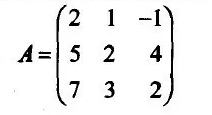
\includegraphics[width=0.25\textwidth]{1.PNG}
  \caption{Квадратная матрица А}\label{fig:par}
\end{figure}


\section{Ход работы}
\subsection{Программа}
Код выполненной программы:
\begin{minted}[caption={Python code}]{python}
import numpy as np

def gauss_inverse(matrix):
    n = len(matrix)
    augmented_matrix = np.concatenate((matrix, np.identity(n)), axis=1)

    print("Исходная матрица A:")
    print(matrix)

    for i in range(n):
        max_index = i
        max_value = augmented_matrix[i, i]
        for j in range(i+1, n):
            if augmented_matrix[j, i] > max_value:
                max_index = j
                max_value = augmented_matrix[j, i]
        augmented_matrix[[i, max_index]] = augmented_matrix[[max_index, i]]
        
        if augmented_matrix[i, i] == 0:
            print("Матрица A является вырожденной. Обратной матрицы не существует.")
            return None
        
        augmented_matrix[i] = augmented_matrix[i] / augmented_matrix[i, i]
        
        print("Преобразование " + str(i+1) + ":")
        print(np.around(np.concatenate((np.identity(n), augmented_matrix[:, n:]), axis=1), decimals=decimals))
        
        for j in range(n):
            if j != i:
                augmented_matrix[j] = augmented_matrix[j] - augmented_matrix[j, i] * augmented_matrix[i]
    
    inverse_matrix = augmented_matrix[:, n:]
    
    return inverse_matrix

# Выбор режима ввода матрицы
mode = input("Выберите способ ввода матрицы:\n1. Сгенерировать случайную матрицу\n2. Ввести матрицу вручную\nВведите число: ")

# Генерация случайной матрицы
if mode.lower() == "1":
    # Ввод размерности матрицы с клавиатуры
    n = int(input("Введите размерность матрицы A: "))
    
    # Генерация случайной матрицы с целыми числами
    matrix = np.random.randint(low=1, high=10, size=(n, n))
    
    print("Сгенерированная матрица A:")
    print(matrix)

# Ввод матрицы вручную
elif mode.lower() == "2":
    # Ввод размерности матрицы с клавиатуры
    n = int(input("Введите размерность матрицы A: "))
    
    # Ввод элементов матрицы с клавиатуры
    print("Введите элементы матрицы A:")
    matrix = np.zeros((n, n), dtype=float)
    for i in range(n):
        for j in range(n):
            matrix[i, j] = float(input("Элемент [" + str(i+1) + ", " + str(j+1) + "]: "))
    
else:
    print("Некорректный выбор режима.")
    exit()

decimals = int(input("Введите количество знаков после запятой для вывода матрицы: "))

inverse = gauss_inverse(matrix)

if inverse is not None:
    print("Обратная матрица A^(-1):")
    print(np.around(inverse, decimals=decimals))
\end{minted}

\subsection{Результат работы программы}
Программа работает следующим образом:

\begin{enumerate}
    \item пользователь выбирает способ ввода матрицы: сгенерировать случайную матрицу или ввести матрицу вручную;
    \item в случае выбора режима "1" (генерирование), программа запрашивает размерность матрицы A и генерирует случайную матрицу с целыми числами;
    \item в случае выбора режима "2" (ввод вручную), программа запрашивает размерность матрицы A и последовательно запрашивает элементы матрицы от пользователя;
    \item программа выводит на экран исходную матрицу A;
    \item программа применяет метод исключения неизвестных Гаусса для преобразования матрицы A в единичную матрицу;
    \item при каждом преобразовании программа выводит промежуточные результаты, включая преобразованную матрицу с единичной матрицей справа;
    \item если в процессе преобразования обнаруживается, что матрица A является вырожденной (в строке или столбце только нули), программа выводит сообщение о невозможности вычислить обратную матрицу и завершается;
    \item в случае успешного преобразования, программа выводит полученную обратную матрицу $A^{-1}$;
    \item пользователю предоставляется возможность указать количество знаков после запятой для округления выводимых чисел;
    \item конечный результат представляет собой исходную матрицу A, преобразованную матрицу с единичной матрицей справа и полученную обратную матрицу $A^{-1}$, выводимые на экран.
    \end{enumerate}
    \noindent

В качестве примера работы кода была использована матрица А (Рис. 1.).

Результат работы программы (Рис. 2.):

\begin{figure}[h]
 \centering
 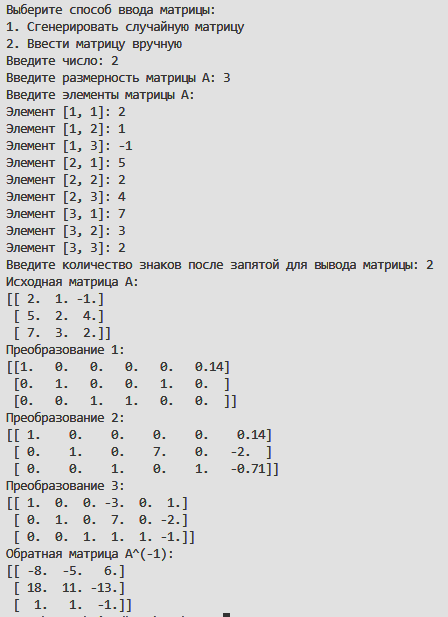
\includegraphics[width=0.7\textwidth]{2.png}
 \caption{Результат работы программы}\label{fig:par}
\end{figure}






\end{document}